\documentclass[a4 paper]{article}
% Set target color model to RGB



\usepackage[inner=2.0cm,outer=2.0cm,top=2.5cm,bottom=2.5cm]{geometry}
\usepackage{setspace}
\usepackage[rgb]{xcolor}
\usepackage{verbatim}
\usepackage{subcaption}
\usepackage{amsgen,amsmath,amstext,amsbsy,amsopn,tikz,amssymb,tkz-linknodes}
\usepackage{fancyhdr}
\usepackage[colorlinks=true, urlcolor=blue,  linkcolor=blue, citecolor=blue]{hyperref}
\usepackage[colorinlistoftodos]{todonotes}
\usepackage{rotating}
%\usetikzlibrary{through,backgrounds}

\usepackage{lmodern}
\usepackage[T1]{fontenc}
\usepackage[capposition=top]{floatrow}
\usepackage{hyperref}
\usepackage{graphicx}
\graphicspath{ {images/} }
\usepackage{booktabs}
\usepackage{changepage}
\usepackage{float}
\usepackage[shortlabels]{enumitem}







\hypersetup{%
pdfauthor={Nick Korbit},%
pdftitle={Homework},%
%pdfkeywords={Tikz,latex,bootstrap,uncertaintes},%
pdfcreator={PDFLaTeX},%
pdfproducer={PDFLaTeX},%
}
%\usetikzlibrary{shadows}
% \usepackage[francais]{babel}
\usepackage{booktabs}


\newcommand{\ra}[1]{\renewcommand{\arraystretch}{#1}}

\newtheorem{thm}{Theorem}[section]
\newtheorem{prop}[thm]{Proposition}
\newtheorem{lem}[thm]{Lemma}
\newtheorem{cor}[thm]{Corollary}
\newtheorem{defn}[thm]{Definition}
\newtheorem{rem}[thm]{Remark}
\numberwithin{equation}{section}

\newcommand{\homework}[6]{
   \pagestyle{myheadings}
   \thispagestyle{plain}
   \newpage
   \setcounter{page}{1}
   \noindent
   \begin{center}
   \framebox{
      \vbox{\vspace{2mm}
    \hbox to 6.28in { {\bf ISYE 6420:~Bayesian Statistics \hfill {\small #2}} }
       \vspace{6mm}
       \hbox to 6.28in { {\Large \hfill #1  \hfill} }
       \vspace{6mm}
       \hbox to 6.28in { {\it Instructor: {\rm #3} \hfill Name: {\rm #5}, gtID: {\rm #6}} }
       %\hbox to 6.28in { {\it TA: #4  \hfill #6}}
      \vspace{2mm}}
   }
   \end{center}
   \markboth{#5 -- #1}{#5 -- #1}
   \vspace*{4mm}
}

\newcommand{\problem}[2]{~\\\fbox{\textbf{Problem #1}}\newline\newline}
\newcommand{\subproblem}[1]{~\newline\textbf{(#1)}}
\newcommand{\D}{\mathcal{D}}
\newcommand{\Hy}{\mathcal{H}}
\newcommand{\VS}{\textrm{VS}}
\newcommand{\solution}{~\newline\textbf{\textit{(Solution)}} }

\newcommand{\bbF}{\mathbb{F}}
\newcommand{\bbX}{\mathbb{X}}
\newcommand{\bI}{\mathbf{I}}
\newcommand{\bX}{\mathbf{X}}
\newcommand{\bY}{\mathbf{Y}}
\newcommand{\bepsilon}{\boldsymbol{\epsilon}}
\newcommand{\balpha}{\boldsymbol{\alpha}}
\newcommand{\bbeta}{\boldsymbol{\beta}}
\newcommand{\0}{\mathbf{0}}



%%%%%%%%%%%%%%%%%%%%%%%%%%%%%%%%%%%%%%%%
%%			 Document				  %%
%%%%%%%%%%%%%%%%%%%%%%%%%%%%%%%%%%%%%%%%


\begin{document}
	
\homework{Midterm Exam}{Spring 2020}{Roshan Vengazhiyil, Brani Vidakovic}{}{Nick Korbit}{903263968}


%%%%%%%%%%%%%%%%%%%%%%%%%%%%%%%%%%%%%%%%
%%			 Problem 1				  %%
%%%%%%%%%%%%%%%%%%%%%%%%%%%%%%%%%%%%%%%%

\problem{1}

We can think about the neurons structure as
a Bayes net. Here we have six binary variables
each of which can take the values of 
``Fire'' and ``Stop''. We could tackle 
the problem the following ways:

\begin{itemize}
	\item Analytical solution;
	\item Full enumeration;
	\item Simulation.
\end{itemize}

As the number of variable is small we'll
start with the \textbf{full enumeration}.
Six binary variables give us 
$2^6=64$ states that system can take.
Since $N_1$ is given a stimulus, 
$P(N_1=Fire)=0.9$. Neurons
$N_2$ to $N_5$ are conditionally dependent 
on the previous neuron. In case
the previous neuron is fired 
$P(N_i=Fire|N_{i-1}=Fire)=0.9$
otherwise $P(N_i=Fire|N_{i-1}=Stop)=0.05$.
Finally, the last neuron is fired 
in case either $N_4$ or $N_5$
is fired 
$P(N_6=Fire|N_4=Fire \lor N_5=Fire)=0.9$
and
$P(N_6=Fire|N_4=Stop \land N_5=Stop)=0.05$.


We develop \textit{run\_full\_enumeration()}
procedure in \textit{neurons.py}. The result 
of the enumeration is a table 
specifying probabilities for 
each of the system's state:

\begin{figure}[H]
	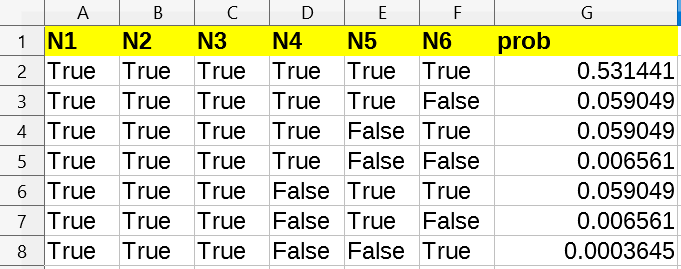
\includegraphics[scale=1.0]{table}
	\centering
	\caption{First 7 entries of the enumeration table.}
	\label{table}
\end{figure}

To calculate the desired probabilities we 
need to sum up the states' probabilities 
where the neurons in question are set 
to $Fire$ (True) or $Stop$ (False).
For example, to calculate $P(N_6=Fire)$
we sum up probabilities from the table 
where $N6=True$. Let's calculate 
the probabilities for parts $a$, $b$ and $c$: 

\begin{enumerate}[a)]
	\item $P(N_6=Fire) \approx 0.8038$
	\item $P(N_6=Fire|N_4=Stop) \approx 0.1353$
	\item $P(N_2=Fire|N_6=Stop) \approx 0.0946$
\end{enumerate}

\textbf{Note}. We interpret ``$N_5$ received stimulus''
as ``previous neuron -- $N_2$ -- is fired''. \newline


It's interesting to contrast 
full enumeration to \textbf{simulation}.
Let's develop a \textit{run\_simulation()}
procedure in \textit{neurons.py} 
and compare results. Running
the simulation for 100000 paths
will yield the following results:

\begin{enumerate}[a)]
	\item $P(N_6=Fire) \approx 0.8039$
	\item $P(N_6=Fire|N_4=Stop) \approx 0.1354$
	\item $P(N_2=Fire|N_6=Stop) \approx 0.0941$
\end{enumerate}






%%%%%%%%%%%%%%%%%%%%%%%%%%%%%%%%%%%%%%%%
%%			 Problem 2				  %%
%%%%%%%%%%%%%%%%%%%%%%%%%%%%%%%%%%%%%%%%

\problem{2}

Since our likelihood is Gamma and
our prior is Gamma, we have a 
conjugate prior problem.
For our Gamma-Gamma case 
the posterior is
also a Gamma, distributed as:

$$
\lambda|\mathbf{X}\sim\mathcal{G}a\left(\alpha+nr,\beta+\sum_{i=1}^{n}X_{i}\right)
$$

Substituting $r=4$, $\alpha=3$, $\beta=5$,
$n=23$ and $\sum_{i=1}^{n}X_{i}=50$ 
we obtain:

$$
\lambda|\mathbf{X}\sim\mathcal{G}a\left(95,171.148\right)
$$

We could calculate Bayes 
estimator as a mean of the resulting
Gamma distribution:

$$
\hat{\lambda}_{b}^{mean}=\frac{\alpha}{\beta}=\frac{95}{171.148}\approx0.555
$$

Let's find the equitailed credible set.
We start with the lower bound $L$:

$$
\int_{-\infty}^{L} \pi(\lambda | x) d \lambda=\alpha / 2
$$

We can substitute the integral with the Gamma cdf:

$$
F_{X}(L) =\alpha / 2
$$

We solve for $L$ numerically using the Brent solver 
implemented via scipy \textit{root\_scalar} function. 

$$
F_{X}(L) - 0.05 / 2 = 0; L\approx 0.4491
$$

Let's turn to the upper bound $U$:

$$
\int_{-\infty}^{U} \pi(\lambda | x) d \lambda= 1 - \alpha / 2
$$

Alternatively

$$
F_{X}(U) = 1 - \alpha / 2
$$

Solving for $U$ gives us:

$$
F_{X}(U) - 1 + 0.05 / 2 = 0; U \approx 0.6721
$$

Resulting in the credible set 
$[0.4491, 0.6721]$ of length $l=0.223$. \newline


Now let's turn to the hypothesis $H_0: \lambda \le 0.5$.
In order to find the probability of $H_0$ we 
integrate the posterior with respect to 
the parameter space:

$$
{p_{0}=\int_{\Lambda_{0}} \pi(\lambda | x) d \lambda=\mathbb{P}^{\lambda | X}\left(H_{0}\right)}
$$

We use posterior $\mathcal{G}a\left(95,171.148\right)$ cdf 
to calculate $p_0$. So that
$$
p_{0}=F_{X}(0.5)\approx 0.1669
$$







%%%%%%%%%%%%%%%%%%%%%%%%%%%%%%%%%%%%%%%%
%%			 Problem 3				  %%
%%%%%%%%%%%%%%%%%%%%%%%%%%%%%%%%%%%%%%%%

\problem{3}

Let $Y_i$ be duration observations,
$\mu_i$ -- the mean and $\tau_i$ -- the 
precision of the Normal distribution:  

$$
\begin{aligned}
	Y_{1}, Y_{2}, \ldots, Y_{n} & \sim \mathcal{N}(\mu, 1 / \tau) \\
	\mu & \sim \mathcal{N}(0.6, 1) \\
	\tau & \sim \mathcal{G}a(20, 0.5)
\end{aligned}
$$

We now find the joint distribution $f(y, \mu, \tau)$;

\begin{align*}
f(y,\mu,\tau)	=\left\{ \prod_{i=1}^{n}f\left(y_{i}|\mu,\tau\right)\right\} \pi(\mu)\pi(\tau)= \\
=	\left\{ \prod_{i=1}^{n}\sqrt{\frac{\tau}{2\pi}}e^{-\tau(y_{i}-\mu)^{2}/2}\right\} \frac{1}{\sqrt{2\pi}}e^{-\frac{1}{2}\left(\mu-0.6\right)^{2}}\frac{0.5^{20}}{\Gamma(20)}\tau^{19}e^{-0.5\tau}
\end{align*}

Removing constant terms will yield us:

$$
f(y,\mu,\tau)\propto\left\{ \prod_{i=1}^{n}\sqrt{\tau}e^{-\tau(y_{i}-\mu)^{2}/2}\right\} e^{-\frac{1}{2}\left(\mu-0.6\right)^{2}}\tau^{19}e^{-0.5\tau}
$$

$$
f(y,\mu,\tau)\propto\tau^{\frac{n}{2}}e^{-\frac{\tau}{2}\sum_{i}^{n}(y_{i}-\mu)^{2}}e^{-\frac{1}{2}\left(\mu-0.6\right)^{2}}\tau^{19}e^{-0.5\tau}
$$


We now find the full conditionals for $\mu$ and $\tau$.
If we look at the priors independently, we 
notice that both Normal-Normal and 
Normal-Gamma are conjugate priors. 
Although Normal-Normal-Gamma is not strictly
a conjugate triplet we can recognize
a semi-conjugate case. We 
derive the following posteriors 
for $\mu$ \cite{miller}:


\begin{align*}
\mu|\tau,y_{1:n}&\sim\mathcal{N}\left(\frac{\tau_{0}\mu_{0}+\tau\sum_{i=1}^{n}y_{i}}{\tau_{0}+n\tau},\left(\lambda_{0}+n\tau\right)^{-1}\right)\\p(\mu_{1}|\tau_{1},y_{1})&=\mathcal{N}\left(\frac{0.6+27.95\tau}{1+43\tau},\left(1+43\tau\right)^{-1}\right)\\p(\mu_{2}|\tau_{2},y_{2})&=\mathcal{N}\left(\frac{0.6+6.48\tau}{1+12\tau},\left(1+12\tau\right)^{-1}\right)
\end{align*}


Knowing that

$$
\sum_{i}^{n}y = n\bar{y}
$$


And posterior for $\tau$:

\begin{align*}
\tau|\mu,y_{1:n}&\sim\mathcal{G}a\left(a+\frac{n}{2},b+\frac{1}{2}\sum\left(y_{i}-\mu\right)^{2}\right)\\p(\tau_{1}|\mu_{1},y_{1})&=\mathcal{G}a\left(41.5,0.5+0.5\left(1.3608+43(0.65-\mu)^{2}\right)\right)\\p(\tau_{2}|\mu_{2},y_{2})&=\mathcal{G}a\left(26,0.5+0.5\left(0.2156+12(0.54-\mu)^{2}\right)\right)
\end{align*}


Knowing that

$$
\sum_{i}^{n}(y_{i}-\mu)^{2}=(n-1)s^{2}+n(\bar{y}-\mu)^{2}
$$


Let's develop a Gibbs sampling procedure
for $\mu$ and $\tau$:

\begin{enumerate}
	\item For $i=1,2$:

	\item Start with $\mu_0=0$, $\tau_0=1$
	
	\item Sample
	\begin{itemize}
		\item $\mu_{n+1}$ from $\mu|\tau,y_{1:n} \sim\mathcal{N}\left(\frac{\tau_{0}\mu_{0}+\tau_n\sum_{i=1}^{n}y_{i}}{\tau_{0}+n\tau_n},\left(\lambda_{0}+n\tau_n\right)^{-1}\right)$
		
		\item $\tau_{n+1}$ from $\tau|\mu,y_{1:n} \sim\mathcal{G}a\left(a+\frac{n}{2},b+\frac{1}{2}\sum\left(y_{i}-\mu_n\right)^{2}\right)$
	\end{itemize}
	
	
	\item Set $n =n+1$ and go to Step 3.
	
\end{enumerate}


We now simulate 11000 samples for $\mu$ and $\tau$ 
for both species. After that we 
calculate the difference $\mu_1-\mu_2$.
Plotting the distribution of the 
resulting sequence will yield us:  

\begin{figure}[H]
	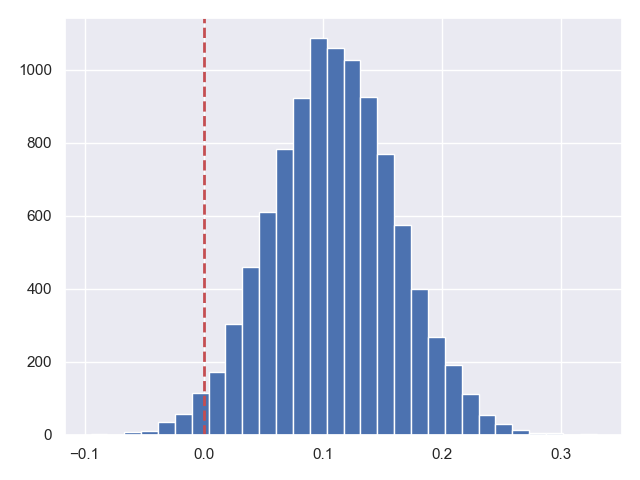
\includegraphics[scale=0.5]{dist}
	\centering
	\caption{Empirical distribution of $\mu_1-\mu_2$.}
	\label{dist}
\end{figure}

The mean of the distribution is 0.1092
with 95\% credible set of $[0.006;0.2136]$.
We also see the red dashed line ($\mu_1-\mu_2=0$)
is visually located far from the 
distribution peak \ref{dist}.
Based on the analysis we can reject 
the hypothesis $H_0: \mu_1=\mu_2$
and conclude that  the length of call is 
indeed a
discriminatory characteristic. \newline



\textbf{Note}. In order to run the code
that solves problems 1 to 3 
sequentially, run the 
command \textit{python runner.py}.
 



%%%%%%%%%%%%%%%%%%%%%%%%%%%%%%%%%%%%%%%%
%%			 Bibliography			  %%
%%%%%%%%%%%%%%%%%%%%%%%%%%%%%%%%%%%%%%%%

\begin{thebibliography}{9}


\bibitem{stat}\label{stat} 
Engineering Biostatistics: An Introduction using MATLAB and WinBUGS. 
Brani Vidakovic - Wiley Series in Probability and Statistics.


\bibitem{miller}\label{miller} 
Bayesian and Modern Statistics. Course material for STA 360/601,
Jeff Miller, Spring 2015, Duke University. Chapter 6: Gibbs Sampling.
\url{https://jwmi.github.io/BMS/chapter6-gibbs-sampling.pdf}

\end{thebibliography}



\end{document} 